% !TeX root = ../thuthesis-example.tex

\chapter{相关工作}

\section{关于共享网络参数的人工神经网络相关研究}
\subsection{迁移学习的研究}

这篇文献\cite{10.1007/978-3-030-01424-7_27}是一篇关于迁移学习的综述。文章中给迁移学习下的定义是给定一个数据集$D_t$和一个学习任务$T_t$,这个学习任务可以从另外一个基于数据集$D_s$的学习任务$T_s$获得帮助,从而加快学习任务$T_t$的学习进程。
这个概念中要解决的问题和我们面临的遗忘问题如出一辙。文中将迁移学习分为四类,即基于对抗的迁移学习,基于网络的迁移学习,基于映射的迁移学习以及基于实例的迁移学习。
其中基于网络的迁移学习提出了共享网络参数来加快目标网络的学习,就是将训练好的神经网络的前若干层的网络结构和参数迁移至新的神经网络,将这些网络连接和学习参数作为新的神经网络的一部分,过程如图\ref{fig:transfer_learning_1}所示。
\begin{figure}
    \centering
    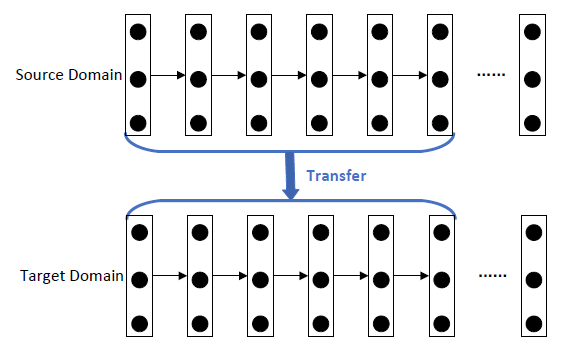
\includegraphics[width=0.9\linewidth]{transfer_learning_1.png}
    \caption{基于网络的迁移学习模型示意图\cite{10.1007/978-3-030-01424-7_27}}
    \label{fig:transfer_learning_1}
\end{figure}

这篇文献\cite{6639081}也采用了相同的思路,实现了语言识别的功能。如图\ref{fig:transfer_learning_2}所示,作者将网络分成两个部分,前一部分是语言独立的特征提取器,最后一层是语言相关的分类器。
神经网络的输入是不同语言的语音片段,经过共享的特征提取器,输出到最后的全连接层。最后全连接层实现将语言分类的功能。文中指出,对于使用欧洲的四种语言训练出来的网络,与使用单个语言训练的网络相比,单词的错误率下降了3\%-5\%。
而对于使用英语和汉语训练出来的网络,与使用单个语言训练的网络相比,单词错误率下降了6\%-28\%。
\begin{figure}
    \centering
    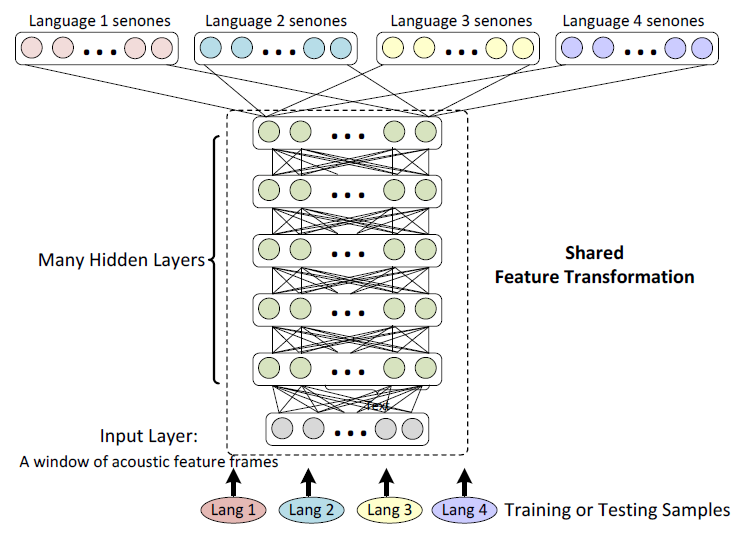
\includegraphics[width=0.9\linewidth]{transfer_learning_2.png}
    \caption{共享特征提取器的语言识别网络\cite{6639081}}
    \label{fig:transfer_learning_2}
\end{figure}

这篇文献\cite{Oquab_2014_CVPR}中讲到了共享特征提取器。如图\ref{fig:transfer_learning_5}所示,网络可以分成两个部分,一部分是卷积层,另一部分是全连接层。
先将网络在一个训练集上训练,训练完成后,将卷积层和若干全连接层迁移到另外一个分类任务当中,替代网络中的卷积层和若干全连接层。
为了更好地适应新的分类任务,作者新增了两层全连接层,然后使用新的训练集对网络进行训练,训练的同时冻结迁移过来的参数,只训练新增的全连接层参数。训练至收敛后,网络同样取得了很好的效果。 
\begin{figure}
    \centering
    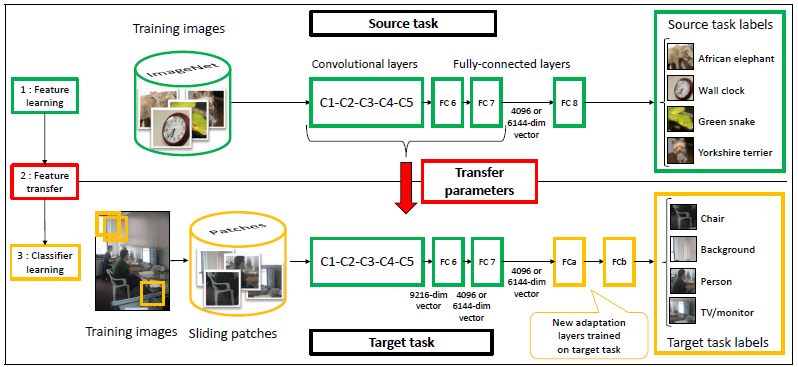
\includegraphics[width=0.9\linewidth]{transfer_learning_5.png}
    \caption{共享特征提取器的卷积神经网络\cite{Oquab_2014_CVPR}}
    \label{fig:transfer_learning_5}
\end{figure}

这篇文献\cite{yosinski_2014_NIPS}对深度神经网络特征可共享的特性进行了研究。如图\ref{fig:transfer_learning_3}所示,第一行代表用数据集1训练的网络,第二行代表用数据集2训练的网络。
第三行代表将前三层参数进行训练,其中实验将冻结参数和不冻结参数分开进行。在训练之前,先将第二行前三层的参数迁移至第三行前三层参数。第四行代表前三层参数使用第一行训练好的前三层参数,之后将这三层参数进行训练,冻结参数和不冻结参数也是分开进行。
最终的结果如图\ref{fig:transfer_learning_4}所示,使用不冻结参数方法的一组,并且使用不同数据集训练的网络得到了很好的泛化效果。从这个实验中可以看出,深度神经网络前若干层参数是可以共享的。
\begin{figure}
    \centering
    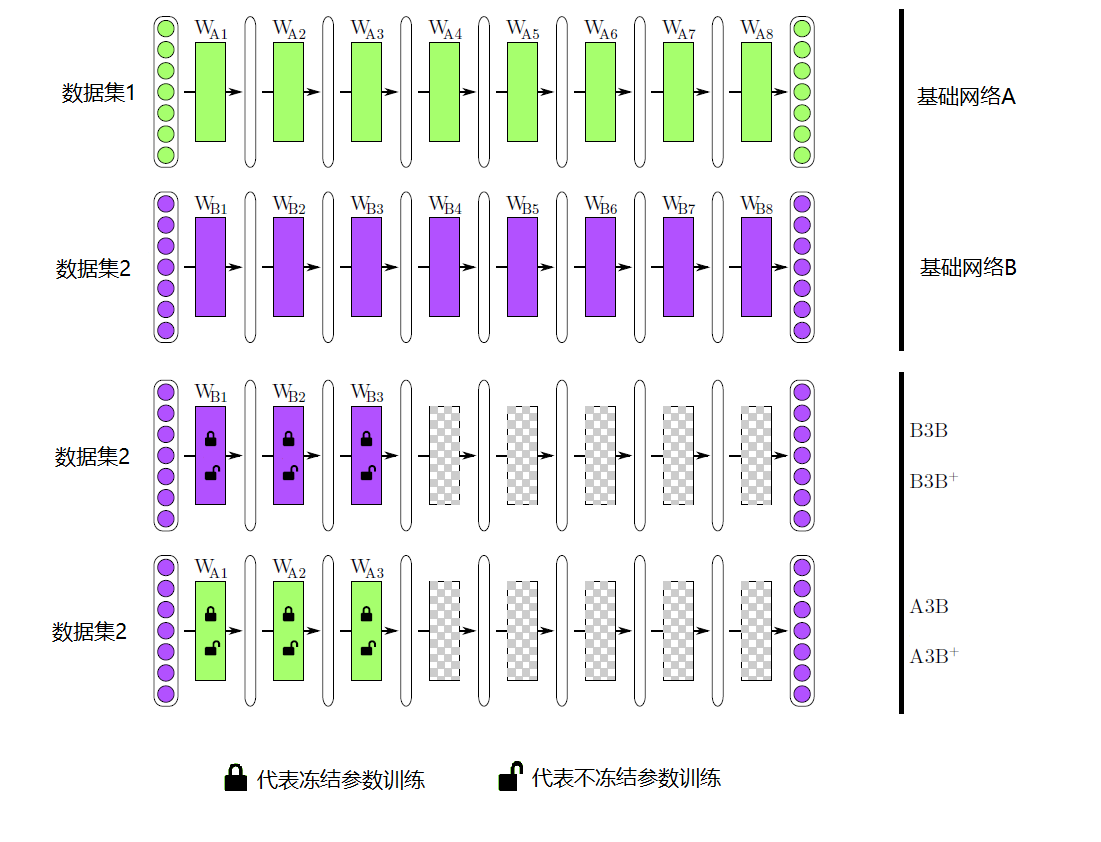
\includegraphics[width=0.9\linewidth]{transfer_learning_3.png}
    \caption{共享参数的深度神经网络训练示意图\cite{yosinski_2014_NIPS}}
    \label{fig:transfer_learning_3}
\end{figure}
\begin{figure}
    \centering
    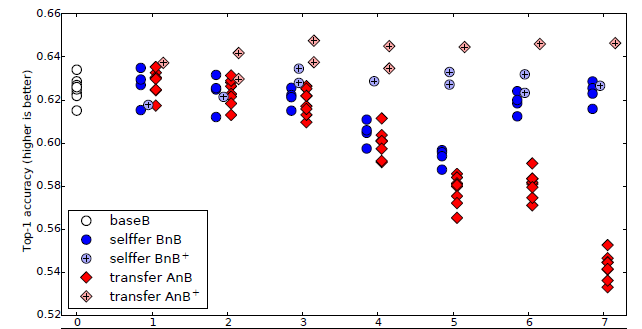
\includegraphics[width=0.9\linewidth]{transfer_learning_4.png}
    \caption{共享参数后实验结果\cite{yosinski_2014_NIPS}}
    \label{fig:transfer_learning_4}
\end{figure}

\subsection{增量学习的研究}
增量学习是指已经学习完成的机器学习模型继续学习新数据的方法。增量学习面临的困难是灾难性遗忘,在已经学习完成的机器学习模型上只用新的数据集去训练会出现旧的分类测试准确率下降的情况。这种情况就好像是学习了新的知识后将旧的知识忘记了一样,因此称为灾难性遗忘。
为了克服灾难性遗忘,这篇综述\cite{PARISI201954}中提到增量学习大致可分为三种类型:基于正则化的方法,基于动态结构的方法以及基于补充学习系统和记忆重放的方法。其中,基于动态结构的方法对本文启发较大。

这篇文献\cite{8107520}对增量学习的方法进行了分类。如图\ref{fig:incremental_learning_1}所示,图中展示了一个已经学习完成的网络在遇到新的学习任务时可能的学习方法。
(a)中是原来已经学习好的模型,前半部分是卷积神经网络,后半部分是全连接层。当加入一个新的类别后,大概有三种可能的解决方法。一种是微调(fine-tuning),即在原来的网络上用新的训练数据直接训练。这样的方法会导致灾难性遗忘。
第二种方法是联合训练(Joint Training),就是用新的训练数据和旧的训练数据同时训练原有的网络。这样带来的效果是比较好的,但是重新训练的成本是很大的。
第三种方法是特征提取(Feature Extraction)的方法。和以前训练好的网络分享一部分参数,这部分参数不用来更新,然后用新的训练数据继续训练没有被冻结的参数。这样的方法可能的问题是新的训练数据也具有自己独特的数据特征,这样的特征由于网络参数的冻结而无法被原有网络提取,因此最终的效果也不会很好。
\begin{figure}
    \centering
    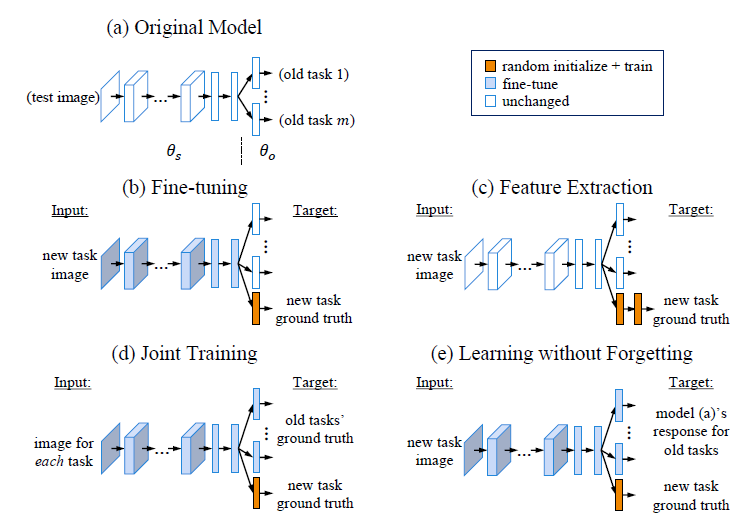
\includegraphics[width=0.9\linewidth]{incremental_learning_1.png}
    \caption{增量学习方法分类\cite{8107520}}
    \label{fig:incremental_learning_1}
\end{figure}

文献\cite{Sarwar_2020}通过共享网络层次,建立新网络分支来解决灾难性遗忘的问题。如图\ref{fig:incremental_learning_2}所示,原来的网络已经训练了50个类别,当有10个新的类别需要添加到网络中时,首先确定好共享网络的层次,然后冻结共享网络和原来分类网络的参数,最后只用新的训练数据对新增加的网络进行训练。
当需要做预测时,将两个网络的输出综合起来,判断应当输出的结果。这样的网络随着新增的类别不断增多而逐渐变得庞大。但是我们从中可以借鉴到共享网络参数的思想。
\begin{figure}
    \centering
    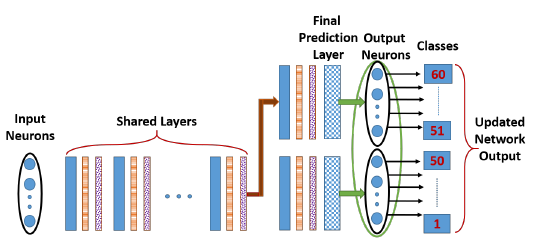
\includegraphics[width=0.9\linewidth]{incremental_learning_2.png}
    \caption{共享网络参数的增量学习\cite{Sarwar_2020}}
    \label{fig:incremental_learning_2}
\end{figure}

\section{关于机器学习模型遗忘方法的研究}
\subsection{非神经网络的遗忘方法}
文献\cite{yinzhicao2015}最早引入了机器学习遗忘的研究,文献使用了统计查询学习\cite{10.1145/293347.293351}的方法对基于贝叶斯方法的机器学习进行了遗忘算法的设计。基于贝叶斯模型的遗忘方法还有文献\cite{10.1145/3196494.3196517}。
文献\cite{antonio2019}对于k-means机器学习的方法设计了遗忘某一个类别的算法。文献\cite{10.1007/978-3-319-40159-1_19}提出了一种基于决策树的遗忘算法。

\subsection{基于神经网络的遗忘方法}
文献\cite{2019arXiv191203817B}提出了一种可以用在神经网络上的遗忘方法。作者首先将训练数据集分成若干互不相交的部分,然后利用每个部分单独训练出一个神经网络模型。网络最终输出的结果将多个神经网络模型输出的结果综合起来,最终输出一个结果。
遗忘的时候,只需要重新训练要遗忘的训练样例所在的神经网络,而无需重新训练所有神经网络模型,过程如图~\ref{fig:machine_unlearning}所示。这样的方式虽然能够使重新训练的工作量减少,但仍未摆脱重新训练的模式,而且训练如此多的神经网络也造成了参数的浪费。
\begin{figure}
    \centering
    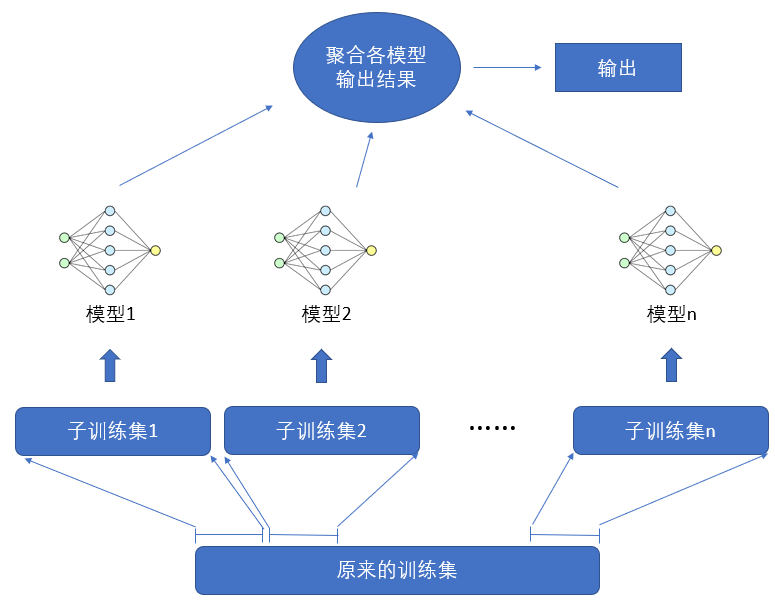
\includegraphics[width=0.9\linewidth]{machine_unlearning.png}
    \caption{将数据集分成若干互不相交集合分别训练\cite{2019arXiv191203817B}}
    \label{fig:machine_unlearning}
\end{figure}
\begin{figure}
    \centering
    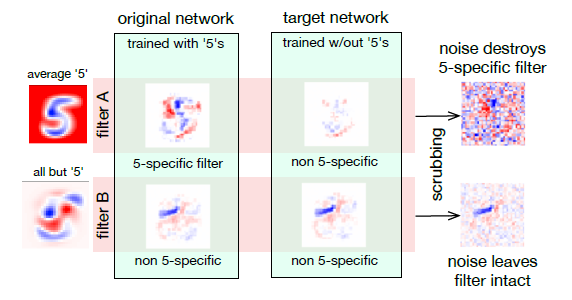
\includegraphics[width=0.9\linewidth]{eternal_sunshine.png}
    \caption{基于增加噪音和正则化的遗忘方法\cite{2019arXiv191203817B}}
    \label{fig:eternal_sunshine}
\end{figure}

这篇文献\cite{Golatkar_2020_CVPR}实现了一种通过在权重上增加噪音的方法来逐渐减少神经网络参数对遗忘数据的信息量,如图~\ref{fig:eternal_sunshine}所示。这篇文献提出了一些值得借鉴的衡量遗忘效果的指标,比如遗忘集的测试准确率,保留集的测试准确率。
文献中还提出了模型置信指标,就是计算目标神经网络与此文方法遗忘之后的网络在遗忘集和保留集上的交叉熵。这些指标在实际应用上具有参考价值,因此本文也参考了这些评价指标。
文献中还提到了一种信息论领域常用到的信息边界衡量方法,就是计算两个网络模型参数的KL散度距离(Kullback-Leibler Divergence)。这种方法经常用于量化两个随机变量概率分布的相似性。
然而,遗忘的目的并不只是简单地让网络的参数去接近目标网络,而是在实际效果上看两个网络的输出是否相近。因为思路上有本质的不同,所以这个衡量指标并没有被本文所采用。这个方法虽然在遗忘的效果上达到了较为理想的状态,然而保留类别的准确率并不是很理想。

这篇文献\cite{Golatkar_2021_CVPR}是神经网络遗忘方向较新的工作。文献中提出了一种混合训练模型,将训练集分为核心训练集和用户训练集。核心训练集表示学习后不会被遗忘的训练集,用户训练集代表学习后可能会被用户遗忘的训练集。文章中使用了两个神经网络用来训练。
第一个网络只用核心训练集进行训练,第二个网络使用第一个网络的输出结果和用户训练集与核心训练的合集一起训练。
为了达到遗忘的效果,这个方法在网络权重上加了随机噪声。文章使用的遗忘指标是遗忘集、保留集和测试集的准确率、重新学习时间、激活距离还有成员推断攻击的成功率。
激活距离定义为目标遗忘网络和这个方法遗忘后的网络对测试集输出差的第一范数值。成员推断攻击的目的是对于给定一个输入,通过一些方法和手段来判断这个输入是否被用于训练网络。其准确率被文献用来当作评价遗忘效果的一个指标。本文借鉴了激活距离这个评价指标。

关于神经网络遗忘算法的相关工作仍有很多种思路,如这两篇文献\cite{10.1007/978-3-030-58526-6_23,pmlr-v119-guo20c}使用牛顿更新的方法。这篇\cite{pmlr-v130-izzo21a}基于影响函数\cite{pmlr-v70-koh17a,cook_weisberg_1982}的思路。
这篇\cite{pmlr-v119-wu20b}是利用将训练过程的存储数据进行参数还原。这篇\cite{pmlr-v132-neel21a}是通过增加噪声实现遗忘。这篇\cite{10.1145/3319535.3363226}是利用反向更新梯度的方法实现异常检测模型检测的还原。
这些思路均没有针对卷积神经网络进行设计算法,也没有充分利用卷积神经网络的特性。

\section{本章小结}
本章首先介绍了关于网络参数共享方面的人工神经网络的相关研究,主要列举了迁移学习领域基于网络的迁移学习方向的相关工作和增量学习研究领域中关于网络参数共享方面的相关工作。
然后介绍了机器学习模型遗忘方法的相关研究工作情况。其中首先介绍了和神经网络无关的机器学习模型的遗忘方法。然后列举了一些基于神经网络的遗忘方法。